Vyšetřete průběh následujících funkcí:

\begin{enumerate}

	%\item  $f(x)=x^3-12x+16$
	%\item  $f(x) = \frac{x^2-1}{x^3-1}$

	\item  $f(x) = \ln(|x| - x^2)$

		\solution{
			Funkce $f$ je sudá, tedy $f(x) = f(-x)$ pro každé $x$ z definičního oboru (ta rovnost znamená že jedna strana je definovaná právě když je ta druhá strana definovaná).

			\begin{itemize}

				\item  \textbf{Definiční obor:} Logaritmus je definován jen pro kladná čísla, tedy
					\begin{align*}
						|x| - x^2 &> 0 \\
						x \in (-1, 0) \cup (0, 1)
					\end{align*}

				\item  \textbf{Spojitost:}
					Na obou intervalech je $f$ spojitá (věta o složení spojitých funkcí a o aritmetice spojitých funkcí).

				\item  \textbf{Limity v krajních bodech:}
					\begin{align*}
						\lim_{x \rightarrow 0^+} \ln(|x| - x^2) &= \lim_{x \rightarrow 0^+} \ln(x(1-x)) \\
						&= -\infty
					\end{align*}
					\begin{align*}
						\lim_{x \rightarrow 1^-} \ln(|x| - x^2) &= \lim_{x \rightarrow 1^-} \ln(x(1-x)) \\
						&= -\infty
					\end{align*}

				\item  \textbf{Derivace:} Pro $x > 0$
					\begin{align*}
						\left( \ln(x-x^2) \right)' &= \frac{1-2x}{x-x^2}
					\end{align*}
					Derivace je definovaná na celém definičním oboru $f$.

				\item  \textbf{Kde je derivace nulová:}
					$f'(x) = 0$ právě pro $x = 1/2$.

				\item  \textbf{Extrémy:}
					Pro $x \in (0, 1/2)$ platí $f'(x) > 0$, tedy $f$ je tam rostoucí.

					Pro $x \in (1/2, 1)$ platí $f'(x) < 0$, tedy $f$ je tam klesající.

					Tedy v $x = 1/2$ je lokální maximum (které je i globálním maximem).

				\item  \textbf{Konvexita, konkavita:}
					Kde je druhá derivace záporná, tam je funkce konkávní.
					$f''(x) = \frac{-2x^2 + 2x - 1}{(x-1)^2x^2} = -\frac{1}{x^2} - \frac{1}{(x-1)^2} < 0$

				\item  \textbf{Graf:} Obrázek~\ref{fig:log_absx_minux_xsquared}.

			\end{itemize}
			\begin{figure}[H]
				\centering
				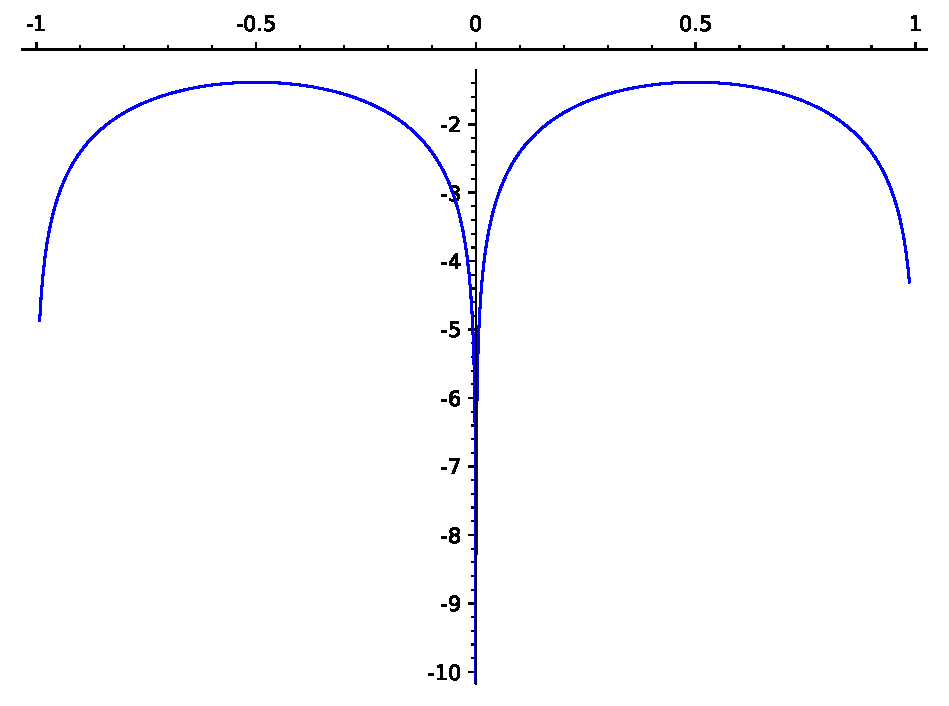
\includegraphics{cviceni_10/fig/log_absx_minus_xsquared.pdf}
				\caption{Graf funkce $\ln(|x| - x^2)$}
				\label{fig:log_absx_minux_xsquared}
			\end{figure}
		}

	\item  $\sin(\sin(x))$

		\solution{
			\url{https://kam.mff.cuni.cz/~sbirka/show_exercise.php?c=93&e=579}
		}

	\item  Spoustu dalších příkladů a jejich řešení na průběh funkce najdete na stránkách Jardy Hančla:

		\url{https://kam.mff.cuni.cz/~jaroslav/vyuka\%2019-20/Cviceni\%20MA1.html}

\end{enumerate}

